\subsection{Método}

O método proposto foi dividido em três fluxos principais: \textit{hardware}, \textit{software} embarcado e modelo preditivo. Essa divisão se justifica porque as seis etapas definidas podem ser desenvolvidas de forma paralela, convergindo, ao final, para a etapa de testes e resultados. A Figura~\ref{fig:fluxogramaMetodo} apresenta o fluxo geral do método.

\begin{figure}[ht]
	\centering
	\caption{Fluxo geral do método proposto.}
	\label{fig:fluxogramaMetodo}
	\definecolor{flowhead}{RGB}{47,63,112}%
	\definecolor{flowbox}{RGB}{234,240,250}%
	\definecolor{flowborder}{RGB}{120,144,190}%
	\definecolor{flowbar}{RGB}{127,131,138}%
	\definecolor{flowint}{RGB}{225,233,245}%
	\definecolor{flowcross}{RGB}{198,93,38}%
	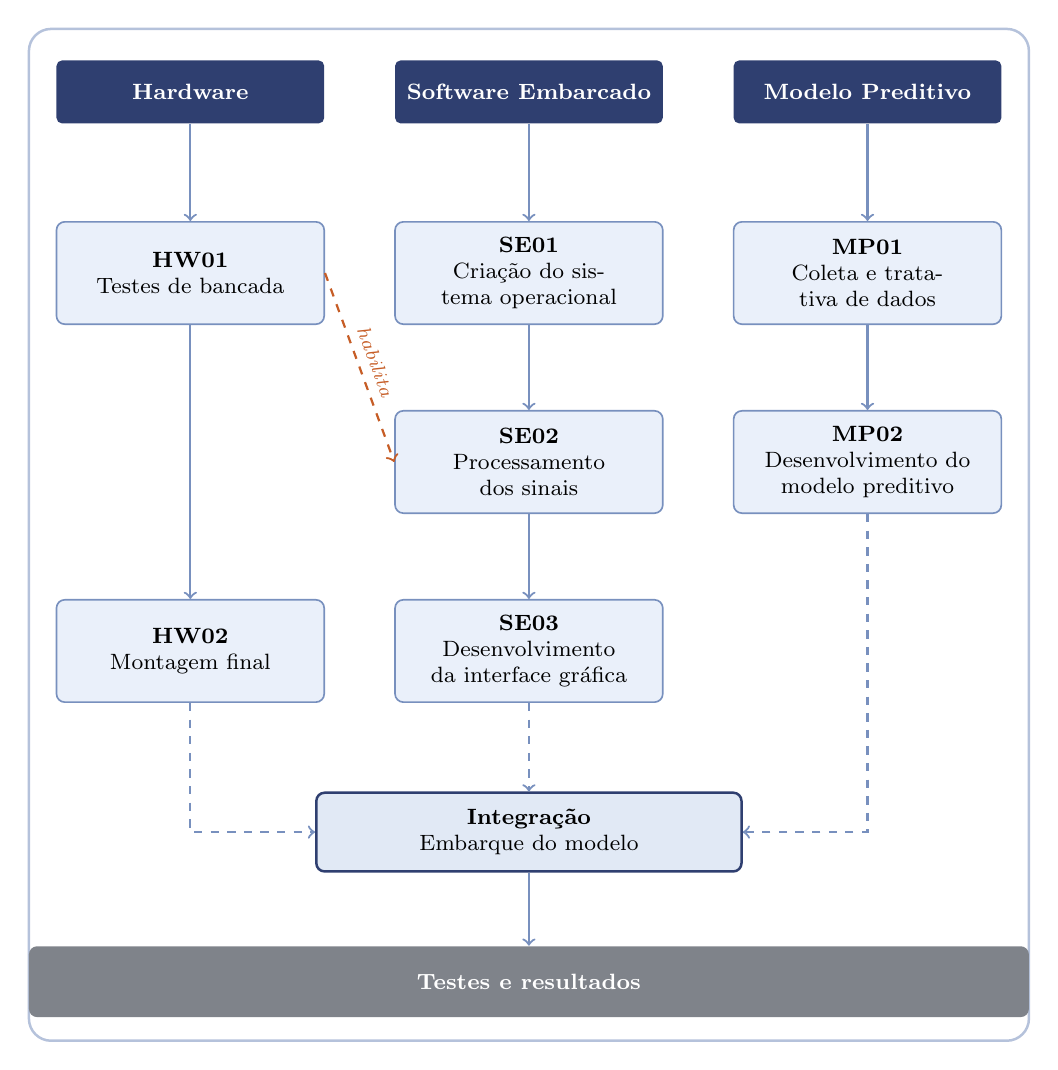
\begin{tikzpicture}[
		font=\footnotesize,
		header/.style={rectangle, rounded corners=2pt, fill=flowhead, text=white,
			font=\footnotesize\bfseries, align=center,
			minimum width=3.4cm, minimum height=0.8cm},
		fstep/.style={rectangle, rounded corners=3pt, draw=flowborder, line width=0.6pt,
			fill=flowbox, align=center, text width=3.0cm,
			minimum width=3.4cm, minimum height=1.3cm, inner sep=3pt},
		fint/.style={rectangle, rounded corners=3pt, draw=flowhead, line width=0.9pt,
			fill=flowint, align=center, text width=5.0cm,
			minimum width=5.4cm, minimum height=1.0cm, inner sep=4pt},
		bar/.style={rectangle, rounded corners=3pt, fill=flowbar, text=white,
			font=\footnotesize\bfseries, align=center, minimum height=0.9cm},
		seq/.style={->, thick, draw=flowborder},
		conv/.style={->, thick, draw=flowborder, dashed},
		xdep/.style={->, thick, draw=flowcross, dashed}
	]
		\draw[rounded corners=8pt, draw=flowborder!55, line width=0.9pt]
			(-2.05,0.8) rectangle (10.65,-12.05);
		% cabeçalhos
		\node[header] (hHW) at (0,0) {Hardware};
		\node[header] (hSE) at (4.3,0) {Software Embarcado};
		\node[header] (hMP) at (8.6,0) {Modelo Preditivo};
		% linha 1
		\node[fstep] (HW01) at (0,-2.3) {\textbf{HW01}\\Testes de bancada};
		\node[fstep] (SE01) at (4.3,-2.3) {\textbf{SE01}\\Criação do sistema operacional};
		\node[fstep] (MP01) at (8.6,-2.3) {\textbf{MP01}\\Coleta e tratativa de dados};
		% linha 2
		\node[fstep] (SE02) at (4.3,-4.7) {\textbf{SE02}\\Processamento dos sinais};
		\node[fstep] (MP02) at (8.6,-4.7) {\textbf{MP02}\\Desenvolvimento do modelo preditivo};
		% linha 3
		\node[fstep] (HW02) at (0,-7.1) {\textbf{HW02}\\Montagem final};
		\node[fstep] (SE03) at (4.3,-7.1) {\textbf{SE03}\\Desenvolvimento da interface gráfica};
		% integração + barra final
		\node[fint] (INT) at (4.3,-9.4) {\textbf{Integração}\\Embarque do modelo};
		\node[bar, minimum width=12.7cm, text width=12.3cm] (TST) at (4.3,-11.3) {Testes e resultados};
		% cabeçalho -> primeira etapa
		\draw[seq] (hHW) -- (HW01);
		\draw[seq] (hSE) -- (SE01);
		\draw[seq] (hMP) -- (MP01);
		% sequência dentro das trilhas
		\draw[seq] (HW01) -- (HW02);
		\draw[seq] (SE01) -- (SE02);
		\draw[seq] (SE02) -- (SE03);
		\draw[seq] (MP01) -- (MP02);
		% dependência entre trilhas: bancada habilita os drivers
		\draw[xdep] (HW01.east) -- node[pos=0.5, sloped, above, font=\scriptsize\itshape, text=flowcross]{habilita} (SE02.west);
		% convergência para a Integração
		\draw[conv] (HW02.south) |- (INT.west);
		\draw[conv] (SE03) -- (INT);
		\draw[conv] (MP02.south) |- (INT.east);
		% integração -> testes
		\draw[seq] (INT) -- (TST);
	\end{tikzpicture}\\
	\textbf{\footnotesize Fonte: Elaborado pelos autores.}
\end{figure}

\textbf{Etapa HW01:} a etapa de testes de bancada consistiu na validação individual de cada componente diretamente sobre a Raspberry Pi 3B+, antes da integração física do dispositivo. Cada sensor foi conectado isoladamente à placa por meio de uma protoboard, o que permitiu verificar a comunicação, a integridade dos sinais e o comportamento elétrico sem a complexidade da montagem completa. O MAX30102 foi validado pelo barramento I\textsuperscript{2}C, confirmando-se o endereçamento do dispositivo e a aquisição do sinal PPG bruto; o DS18B20 foi verificado pelo barramento 1-Wire, incluindo a checagem do resistor de \textit{pull-up} exigido pelo protocolo; os periféricos de alerta, \textit{buzzer} e LED RGB, foram testados via GPIO, e o \textit{display}, pelas interfaces de vídeo e toque. Para cada teste foram desenvolvidos programas em C++ que exercitaram a leitura e o controle dos componentes; esses programas validaram os \textit{drivers} de comunicação e foram posteriormente reaproveitados como base do processo principal da aplicação, desenvolvido em C++ com o \textit{framework} Qt. Essa abordagem incremental de \textit{bring-up} reduziu o risco da etapa de integração, isolando problemas de comunicação ou de configuração ainda na bancada.

\textbf{Etapa HW02:} validados os componentes individualmente, realizou-se a montagem final do protótipo, consolidando a fiação e fixando os elementos no invólucro impresso em PETG. As ligações provisórias de bancada foram substituídas por conexões definitivas e organizadas, reduzindo a probabilidade de mau contato durante a operação contínua. A alimentação partiu de uma fonte chaveada de 5 V conectada a um barramento de distribuição, a partir do qual a Raspberry Pi, o \textit{display} e os ventiladores foram alimentados em paralelo, evitando que toda a corrente trafegasse pela placa de processamento; os sensores e os periféricos de alerta, de baixo consumo, foram alimentados diretamente pelos pinos da Raspberry Pi. Para a gestão térmica, exigida pela operação contínua sob carga de inferência, foram previstos quatro ventiladores: dois de pequeno porte dedicados ao processador e dois maiores para o fluxo de ar interno do invólucro. A fonte foi dimensionada para o consumo agregado desses elementos. O resultado é o dispositivo integrado, fisicamente fechado e pronto para a execução conjunta do \textit{software} embarcado e do modelo preditivo.

\textbf{Etapa SE01:} a primeira etapa do \textit{software} embarcado consistiu na construção da imagem do sistema operacional sobre a qual a aplicação é executada, gerada com o Buildroot a partir da configuração base da Raspberry Pi 3B+. O Buildroot foi adotado por produzir, a partir de uma \textit{toolchain} de compilação cruzada, uma imagem Linux enxuta e reprodutível, com controle fino sobre os pacotes incluídos, característica alinhada às restrições de recursos e aos requisitos de confiabilidade de um dispositivo de uso clínico.

A configuração do \textit{kernel} habilitou, por meio de \textit{device tree overlays}, as interfaces exigidas pelos sensores, I\textsuperscript{2}C para o MAX30102 e 1-Wire para o DS18B20, além da saída de vídeo e da entrada por toque do \textit{display}. Sobre uma base mínima de sistema provida pelo BusyBox, a imagem incorporou os pacotes efetivamente necessários à aplicação: o \textit{runtime} da linguagem C++ e as bibliotecas do \textit{framework} Qt para a interface gráfica, os módulos de \textit{kernel} de comunicação (\texttt{i2c-dev}, \texttt{w1-gpio} e \texttt{w1-therm}) e as dependências de execução do modelo preditivo. A seleção foi mantida em um \textit{defconfig} versionado, garantindo a reprodutibilidade do ambiente e reduzindo o tempo de inicialização e a superfície de falhas do sistema.

\textbf{Etapa SE02:} esta etapa abrangeu o \textit{software} responsável pela leitura dos sensores, pelo processamento dos sinais fisiológicos e pelo cálculo do escore NEWS2. A leitura do MAX30102 foi feita pela interface \textit{/dev/i2c} e a do DS18B20, sensor de temperatura corporal, pelo \textit{driver} \textit{w1-therm}, ambos expostos nativamente pelo \textit{kernel} Linux. A partir do sinal PPG, a frequência cardíaca (FC) e a saturação de oxigênio (SpO\textsubscript{2}) foram extraídas de forma direta, respectivamente pela detecção de picos no componente pulsátil e pela razão de absorção entre os comprimentos de onda vermelho e infravermelho \cite{allen2007photoplethysmography}, enquanto a frequência respiratória (FR) foi estimada a partir das modulações respiratórias do sinal \cite{charlton2018breathing}.

A pressão arterial (PA) é o parâmetro de obtenção não invasiva mais complexa a partir do sinal PPG. Por isso, adotou-se a abordagem mais direta e clinicamente confiável: o registro manual do valor pela equipe de enfermagem por meio da interface do equipamento. Como a pressão arterial é empregada de forma intermitente no NEWS2, essa estratégia atende ao protocolo sem depender de estimativas de menor acurácia.

Os cinco parâmetros foram amostrados em janelas de 30 segundos e, ao fim de cada janela, submetidos ao cálculo do NEWS2 conforme as faixas clínicas do protocolo \cite{smith2013news}. O escore resultante alimentou tanto a classificação imediata de risco quanto o modelo preditivo descrito adiante.

\textbf{Etapa SE03:} a etapa de desenvolvimento da interface gráfica construiu, com o \textit{framework} Qt, a camada de interação entre o sistema e a equipe de saúde, exibida no \textit{display} de toque capacitivo acoplado à plataforma. A renderização foi desacoplada da aquisição e do processamento dos sinais, executados em \textit{threads} distintas, de modo a preservar a responsividade da interface mesmo durante o processamento contínuo.

A tela foi organizada em duas regiões. A primeira apresenta os cinco sinais vitais que compõem o NEWS2, cada um com seu valor, unidade e a cor correspondente à faixa de pontuação do protocolo, facilitando identificar qual parâmetro está alterado. A segunda concentra os dois principais indicadores: o escore NEWS2 atual, com sua classificação de risco (baixo, médio ou alto), e o NEWS2 estimado para um horizonte futuro pelo modelo preditivo, que indica a tendência de evolução do paciente e auxilia a equipe a antecipar intervenções. Como elementos auxiliares, a interface contempla a identificação do paciente, o registro temporal da última atualização e indicadores do estado dos sensores, sinalizando eventuais perdas de contato ou falhas de leitura que possam comprometer a confiabilidade dos dados exibidos.

\textbf{Etapa MP01:} para o desenvolvimento e a validação dos modelos preditivos, foi utilizado o conjunto de dados disponibilizado em \cite{REYNA}. A escolha desse conjunto justifica-se por quatro fatores: (i) sua disponibilidade pública, sem necessidade de processo de credenciamento individual, o que favorece a reprodutibilidade do trabalho; (ii) o volume amostral de 40.336 pacientes, suficiente para o treinamento robusto de modelos com alta capacidade representacional; (iii) a presença de séries temporais com periodicidade horária, contendo as variáveis fisiológicas necessárias ao cálculo do NEWS2; e (iv) o caráter multicêntrico, com dados provenientes de dois sistemas hospitalares distintos (Beth Israel Deaconess Medical Center e Emory University Hospital), o que viabiliza estratégias de validação externa.
Cada registro do conjunto corresponde a uma hora de internação de um paciente, e contempla as variáveis fisiológicas FC, SpO\textsubscript{2}, temperatura, pressão arterial sistólica (PAS), pressão arterial diastólica (PAD), pressão arterial média (PAM) e FR, além de exames laboratoriais e dados demográficos.

A variável-alvo dos modelos preditivos é o valor do NEWS2, calculado conforme as faixas e pesos definidos pelo Royal College of Physicians (2017). Para cada registro horário do conjunto de dados, o escore foi computado a partir das colunas FC, SpO\textsubscript{2}, temperatura, PAS e FR, atribuindo-se a cada variável uma pontuação entre 0 e 3 conforme suas faixas fisiológicas, e somando-se as pontuações parciais para obtenção do escore agregado, que varia de 0 a 20.

O conjunto de dados é processado em quatro etapas sequenciais. Primeiramente, realiza-se a filtragem de pacientes, excluindo-se aqueles com menos de $W + h$ horas de registro, uma vez que estes não comportam a montagem da janela mínima de entrada nem a definição da variável-alvo no horizonte considerado. Em seguida, aplica-se a imputação de valores ausentes por meio da técnica \textit{forward-fill} limitada a uma janela de 4 horas, considerando que medições mais antigas perdem representatividade fisiológica. Para cada valor imputado, uma variável binária adicional é criada de forma a sinalizar a imputação ao modelo, preservando a informação implícita contida no padrão de medição --- informação clinicamente relevante, dado que a frequência de aferição é em si um indicador de instabilidade percebida pela equipe assistencial.

Na terceira etapa, são extraídas estatísticas descritivas para cada variável fisiológica dentro da janela $X_{t-W+1:t}$, incluindo média, desvio padrão, valor mínimo, valor máximo, último valor observado e coeficiente angular do ajuste linear sobre a janela. Adiciona-se ainda o valor do NEWS2 calculado para cada um dos $W$ instantes da janela, dado que sua trajetória histórica constitui uma das características mais informativas para a predição, conforme demonstrado por \citeonline{salehinejad}. Por fim, todas as variáveis numéricas são normalizadas por padronização \textit{z-score} utilizando estatísticas estimadas exclusivamente sobre o conjunto de treinamento, de modo a evitar vazamento de informação.

\textbf{Etapa MP02:} são avaliados três modelos com vieses indutivos distintos, selecionados de modo a cobrir um espectro de complexidade e a permitir comparações metodologicamente significativas. A regressão logística, com regularização $L_{2}$, atua como modelo de referência (\textit{baseline}) e como análogo computacional ao próprio NEWS2. O segundo modelo é o XGBoost, um algoritmo de \textit{gradient boosting} sobre árvores de decisão amplamente consagrado em tarefas tabulares com séries temporais clínicas \cite{churpek2016}. Por fim, emprega-se uma rede neural recorrente do tipo LSTM (\textit{Long Short-Term Memory}), aplicada diretamente sobre a sequência de sinais vitais reamostrados. %*possivelmente desconsiderar XgBoost, que é decisão binária.%

A justificativa metodológica para a comparação desses três modelos reside na cobertura de paradigmas indutivos distintos: linear interpretável, \textit{ensemble} de árvores e rede neural sequencial. Essa escolha permite isolar a contribuição de cada classe de viés indutivo para o desempenho preditivo, ao invés de comparar modelos da mesma família, evitando que os resultados reflitam apenas variações de hiperparâmetros dentro de um único paradigma.
